\documentclass[10pt,a4paper]{article}
\usepackage[utf8]{inputenc}
\usepackage{amsmath}
\usepackage{amsfonts}
\usepackage{amssymb}
\usepackage{tikz}
\usepackage{graphicx}
\author{James Lee}
\title{7th Assignment of Computational Physics}
\begin{document}
	\maketitle
	\begin{abstract}
		In this report I present to you the numerical solution to Problem 2.19.
	\end{abstract}
	\section{Introduction}
	This program aims to compute the motion of baseball.\\
	Baseball is a bat-and-ball game played between two teams of nine players each who take turns batting and fielding.\\
	The batting team attempts to score runs by hitting a ball that is thrown by the pitcher with a bat swung by the batter, then running counter-clockwise around a series of four bases: first, second, third, and home plate. A run is scored when a player advances around the bases and returns to home plate.\\
	Players on the batting team take turns hitting against the pitcher of the fielding team, which tries to prevent runs by getting hitters out in any of several ways. A player on the batting team who reaches a base safely can later attempt to advance to subsequent bases during teammates' turns batting, such as on a hit or by other means. The teams switch between batting and fielding whenever the fielding team records three outs. One turn batting for both teams, beginning with the visiting team, constitutes an inning. A game comprises nine innings, and the team with the greater number of runs at the end of the game wins. Baseball is the only major team sport in America with no game clock, although almost all games end in the ninth inning.\\
	Baseball's motion is governed by Newtonian mechanical laws. Therefore, it will not be difficult for us to solve projectile motion. However, one should take air drag effects and Magnus effects into consideration if one wishes to find a rather accurate solution. In the following discussions, I will present to you numerical solutions.
	\subsection{Baseball Dynamics}
	After a baseball is thrown, its motion will only be influenced by gravity and forces exerted by air according to Newton's 2nd Law. It will be elementary for us to write down the ODE that describes the motion\\
	ODE to describe this model:
	\begin{equation}
	m\frac{d^{2}\vec{r}}{dt^2}=\vec{G}-B_{2}v^{2}\vec{e_{v}}+S_{0}\vec{\omega}\times \vec{v}
	\end{equation}
	where $\vec{e_{v}}$ is unit vector in the direction of $\vec{v}$.\\
	Now we want to investigate the backspin case.\\
	We adopt the approximation that:\\
	1. The angular velocity is along $z$-axis all the time.\\
	2. All terms that include $v_z$ vanish.\\
	Component form:
	\begin{align}
	\frac{dx}{dt}&=v_x\\
	m\frac{dv_x}{dt}&=-B_{2}vv_x-S_0\omega_zv_y\\
	\frac{dy}{dt}&=v_y\\
	m\frac{d^{2}y}{dt^{2}}&=-mg-B_{2}vv_y+S_0\omega_zv_x
	\end{align}
	where:
	\begin{align}
	\frac{B_2}{m}&=0.0039+\frac{0.0058}{1+\text{exp}(\frac{v-35}{5})}\\
	\frac{S_0}{m}&=4.1\times 10^{-4}
	\end{align}
	It is not easy to solve this ODE analytically. I will solve it numerically in the following discussions.
	
    \section{Main Content}
    \subsection{The Range of a Batted Ball}
    I will use Euler methods to solve this set of ODE. The program is very much alike the program in Assignment 6. \\
    Firstly, let us fix the initial condition:
    \begin{align}
    x|_{t=0}&=0\\
    y|_{t=0}&=0\\
    v_x|_{t=0}&=v\cos{\pi/4}\\
    v_y|_{t=0}&=v\sin{\pi/4}
    \end{align}
    where:
    \begin{equation}
    v=110\text{ mph}
    \end{equation}     
    The numerical solution to this case will be plotted in figure.1.
    \begin{figure}[htbp]
    	\centering
    	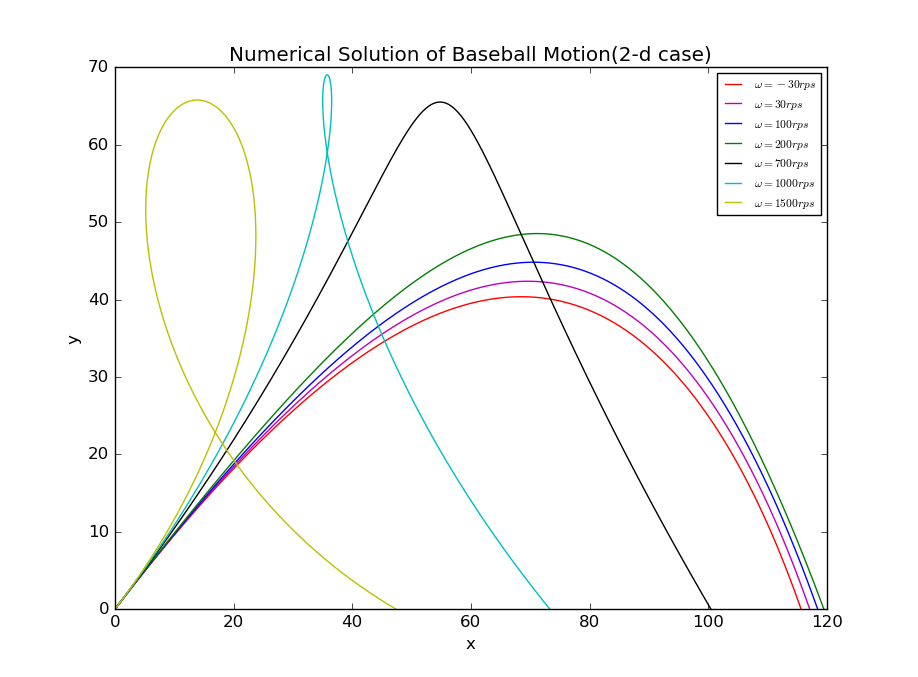
\includegraphics[width=5in]{baseball_1.png}
    	\caption{Numerical Solutions with different $\omega$}
    \end{figure}
    As we can see in the numerical plot figure, the batted baseball motion range increases as angular velocity becomes bigger. However, the baseball motion range begins to decrease after the angular velocity reaches a certain value(in our case, the threshold value is $\omega=231rps$). One should notice that the ball goes higher as angular velocity increases. When having reached a specific value, the baseball's motion begings to show peculiar characteristics: it seems to be blown back by the wind!\\
   \subsection{3-d Motion Case}
   Now we wish to investigate the 3-d motion of baseball.\\
   Thus, we need to alter the angular velocity's direction from $z$-axis to $y$-axis.\\
   Component form:
   \begin{align}
   \frac{dx}{dt}&=v_x\\
   m\frac{dv_x}{dt}&=-B_{2}vv_x\\
   \frac{dy}{dt}&=v_y\\
   m\frac{d^{2}y}{dt^{2}}&=-mg-B_{2}vv_y\\
   \frac{dz}{dt}&=v_z\\
   m\frac{d^{2}z}{dt^{2}}&=-S_0\omega_yv_x
   \end{align}
   the initial conditions are:
   \begin{align}
   x|_{t=0}&=0\\
   y|_{t=0}&=0\\
   z|_{t=0}&=0\\
   v_x|_{t=0}&=v\cos{\theta}\\
   v_y|_{t=0}&=v\sin{\theta}\\
   v_z|_{t=0}&=0\\
   \end{align}
   where
   \begin{equation}
   v=110\text{ mph}
   \end{equation}
   
    \begin{figure}[htbp]
    	\centering
    	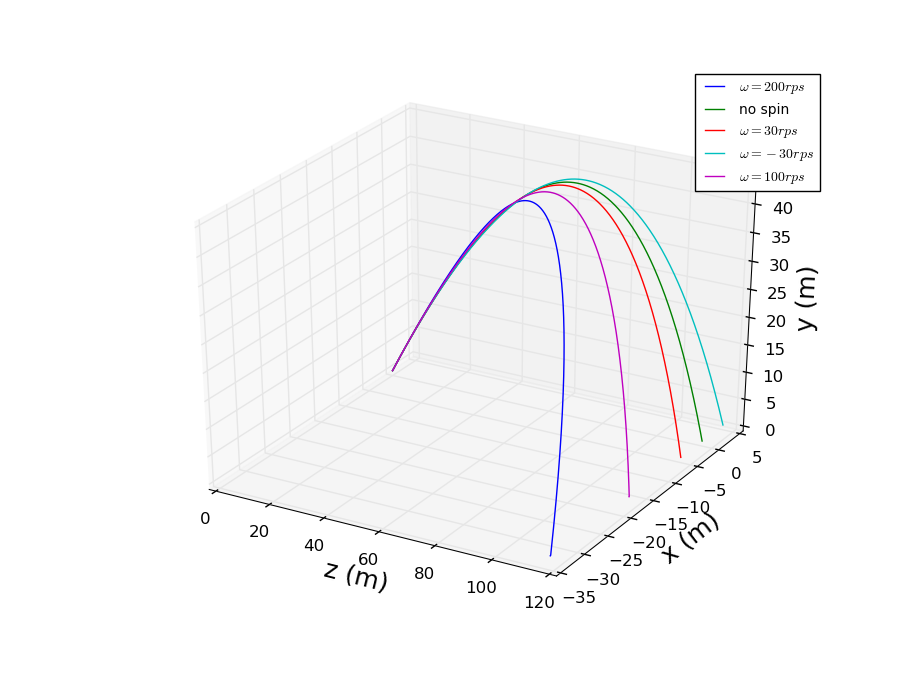
\includegraphics[width=5in]{baseball_2.png}
    	\caption{Numerical Solutions\label{Figure_2}}
    \end{figure}
     The numerical solution to this case will be plotted in figure \ref{Figure_2}.
    As we can see in this figure, the baseball's trajectory will deviate more from the no-spin trajectory when its angular velocity increases. This feature agrees with our common sense.
    
    \section*{Acknowledgement}
    When tackling this assignment, I benefitted a lot from the valuable discussions with Liu Xingchen. I would like to thank him for pointing out several syntax errors I made, also, for his willingness to discuss with me.
    
    \begin{thebibliography}{99}
    	\bibitem{}Hunter J, the Matplotlib Documentation, 2016
    	\bibitem{}Giordano N.J, Nakanishi H, Computational Physics, Pearson Education, 2007
    \end{thebibliography} 
\end{document}